\documentclass[11pt]{article}
\usepackage[T1]{fontenc}
\usepackage[margin=0.92in]{geometry}
\usepackage{amsmath,amssymb,amsthm,mathtools}
\usepackage{graphicx}
\usepackage{microtype}
\usepackage{xcolor}
\usepackage[colorlinks=true,linkcolor=blue!55!black,urlcolor=blue!65!black,citecolor=blue!55!black]{hyperref}

\newtheorem{theorem}{Theorem}
\newtheorem{lemma}[theorem]{Lemma}
\newtheorem{remark}[theorem]{Remark}
\newcommand{\R}{\mathbb R}
\newcommand{\Fdim}{\dim_{\mathrm F}}
\newcommand{\Fspec}{\dim_{\mathrm F}^{\theta}}
\newcommand{\J}{\mathcal J}
\newcommand{\e}{\mathrm e}

\title{Sharp H\"older bounds for the Fourier spectrum:\\
the compact and noncompact answers differ}
\author{Candidate full solution to Question 1.4 of arXiv:2210.07019}
\date{11 August 2026}

\begin{document}
\maketitle

\noindent
\fbox{\begin{minipage}{0.94\textwidth}
\textbf{Status: candidate full solution, likely valid.}
Let $t=\Fdim\mu<\infty$. The general upper bound in Theorem 1.3 of
Fraser,
\[
 \dim_{\mathrm F}^{\theta}\mu
 \le t+d\left(1+\frac{t}{2\alpha}\right)\theta,
 \tag{A}
\]
is sharp for every $d\ge1$, $0<\alpha\le1$, and $t\ge0$: a finite
positive measure with an $\alpha$-H\"older Fourier transform attains
equality for every $0\le\theta\le1$. In contrast, compact support implies
the strictly stronger exact bound
\[
 \dim_{\mathrm F}^{\theta}\mu\le t+d\theta. \tag{B}
\]
For every $t\ge0$, a compactly supported positive measure attains equality
in (B) for every $\theta$. Thus (A) is not sharp in the compactly supported
class when $t>0$, and (B) is the optimal replacement.
\end{minipage}}

\section{The exact question}

For a finite Borel measure $\mu$ on $\R^d$, Fraser defines
\[
 \J_{s,\theta}(\mu)^{1/\theta}
 =\int_{\R^d}|\widehat\mu(\xi)|^{2/\theta}
       |\xi|^{s/\theta-d}\,d\xi \qquad(0<\theta\le1)
\]
and
\(
 \dim_{\mathrm F}^{\theta}\mu
 =\sup\{s\ge0:\J_{s,\theta}(\mu)<\infty\}.
\)
At $\theta=0$ this is the usual Fourier dimension
\[
 \Fdim\mu=\sup\{s\ge0:|\widehat\mu(\xi)|\lesssim |\xi|^{-s/2}\}.
\]
Theorem 1.3 proves (A) whenever $\widehat\mu$ is
\(\alpha\)-H\"older. Question 1.4 asks whether this is sharp, especially
when $\mu$ is compactly supported and $\Fdim\mu>0$ \cite{Fraser}.
The complete source page is reproduced below.

\begin{center}
 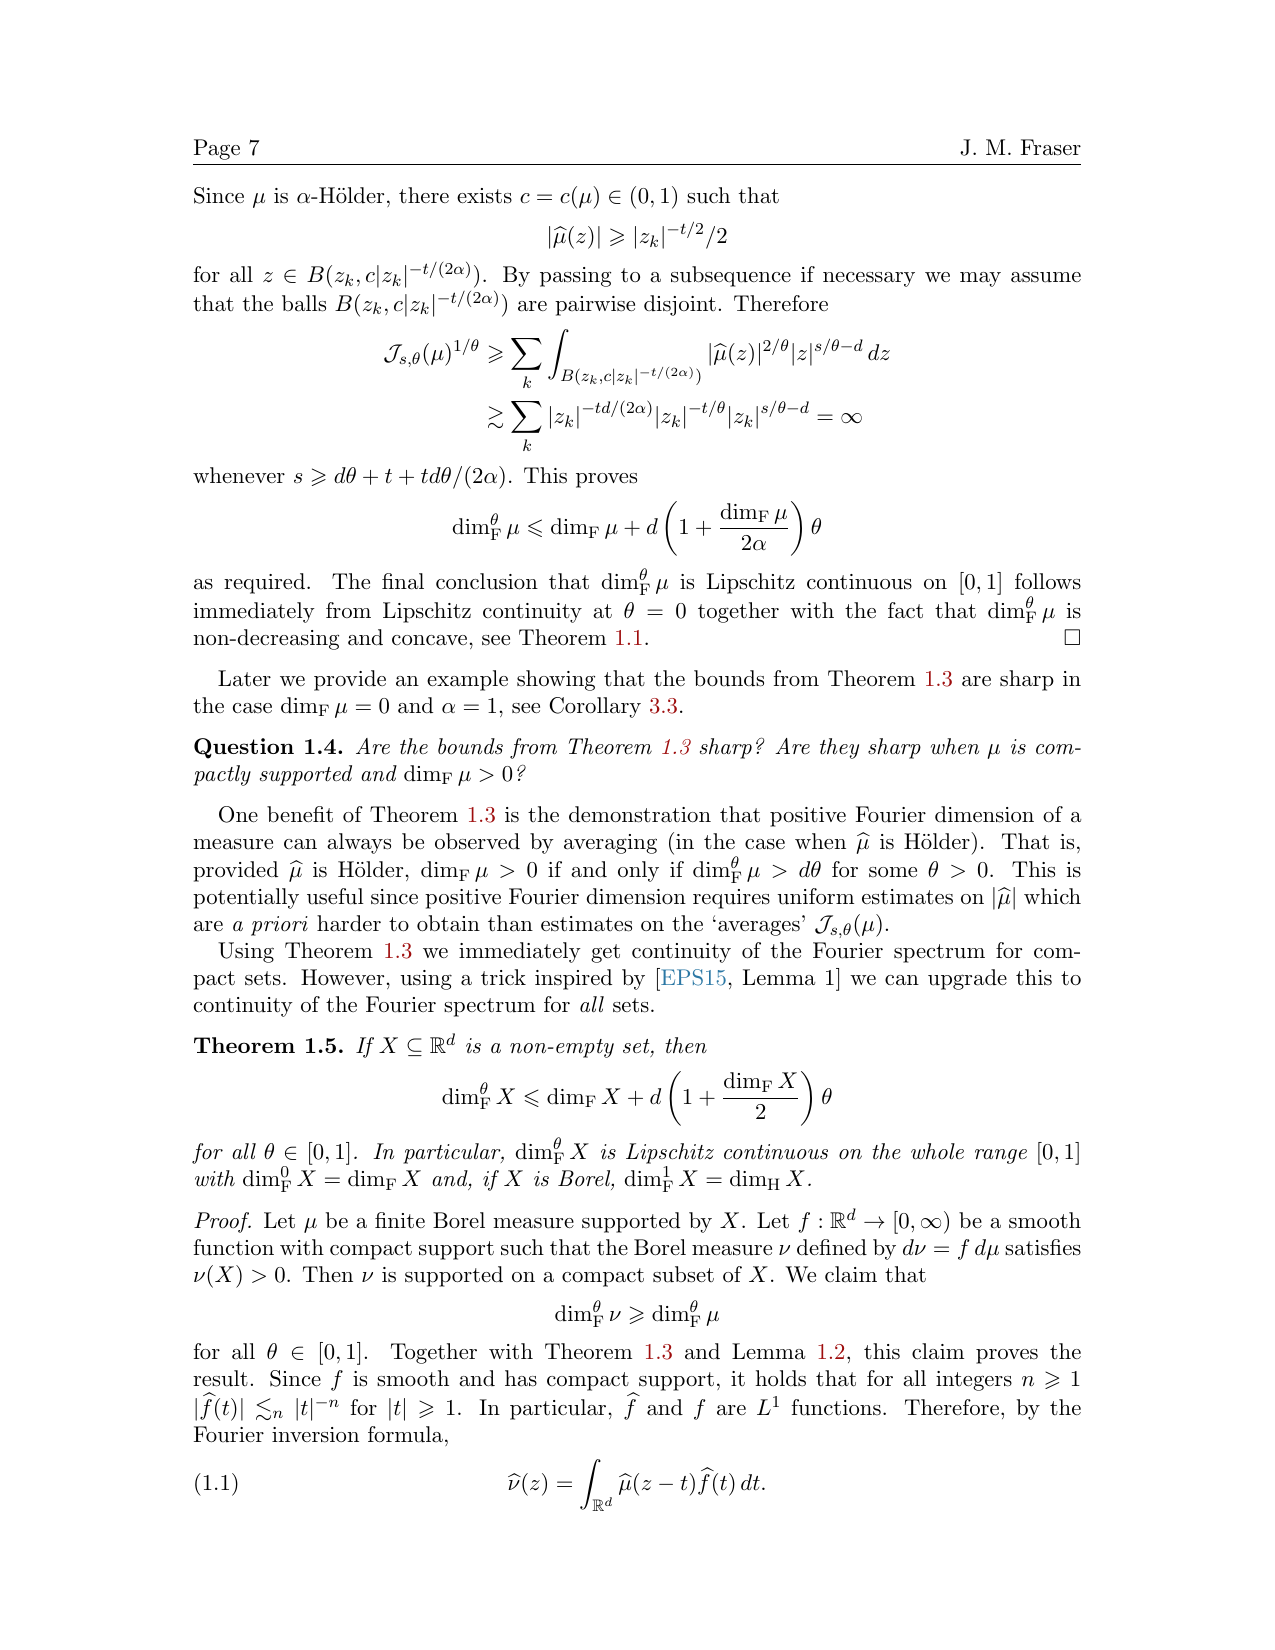
\includegraphics[height=0.73\textheight]{figures/source_page7.png}
\end{center}

\section{Compact support forces a better upper bound}

\begin{theorem}[compact-support bound]\label{thm:compact-upper}
Let $\mu$ be a compactly supported finite Borel measure on $\R^d$ and
let $t=\Fdim\mu<\infty$. Then, for every $0\le\theta\le1$,
\[
 \dim_{\mathrm F}^{\theta}\mu\le t+d\theta.
\]
\end{theorem}

\begin{proof}
The claim at $\theta=0$ is the definition, so fix $\theta>0$. First
suppose $t>0$, and choose $0\le v<t<u$. The definition of Fourier
dimension gives
\begin{equation}\label{eq:subcritical-decay}
 |\widehat\mu(\xi)|\le C_v(1+|\xi|)^{-v/2}.
\end{equation}
Choose $\chi\in C_c^\infty(\R^d)$ equal to one on a neighbourhood of
\(\operatorname{spt}\mu\). For $j=1,\dots,d$,
\[
 \partial_j\widehat\mu=-2\pi i\,\widehat{x_j\mu}
 =-2\pi i\bigl(\widehat{x_j\chi}*\widehat\mu\bigr).
\]
Convolution with a Schwartz function preserves every polynomial decay
estimate, so \eqref{eq:subcritical-decay} implies
\begin{equation}\label{eq:gradient-decay}
 |\nabla\widehat\mu(\xi)|\le C'_v(1+|\xi|)^{-v/2}.
\end{equation}

Since $u>t$, there is a sequence $\xi_k$, with
\(R_k=|\xi_k|\to\infty\), such that
\[
 |\widehat\mu(\xi_k)|\ge R_k^{-u/2}.
\]
The mean-value theorem and \eqref{eq:gradient-decay} show that, for a fixed
small $c>0$,
\begin{equation}\label{eq:large-balls}
 |\widehat\mu(\xi)|\ge\tfrac12R_k^{-u/2}
 \quad\text{when}\quad
 |\xi-\xi_k|\le cR_k^{-(u-v)/2}.
\end{equation}
Pass to a subsequence so that these balls are disjoint. Their contribution
to the energy is bounded below by a constant times
\[
 \sum_k
 R_k^{-u/\theta}
 R_k^{s/\theta-d}
 R_k^{-d(u-v)/2}.
\]
Every summand is bounded below away from zero, and hence the energy
diverges, whenever
\[
 s\ge u+d\theta+\frac{d\theta}{2}(u-v).
\]
Let $u\downarrow t$ and $v\uparrow t$ to obtain
\(\dim_{\mathrm F}^{\theta}\mu\le t+d\theta\).
If $t=0$, the same proof uses $v=0$: boundedness of
\(\widehat\mu\), together with the cutoff identity, gives a bounded
gradient. Letting $u\downarrow0$ gives the same conclusion.
\end{proof}

The gain over Theorem 1.3 is structural. H\"older continuity propagates a
peak of height $R^{-u/2}$ only across a ball of radius
\(R^{-u/(2\alpha)}\). Compact support lets every subcritical decay estimate
propagate to the gradient, enlarging that radius to
\(R^{-(u-v)/2}\); as $u,v\to t$, the radius loses no power of $R$.

\section{A lacunary bump bookkeeping lemma}

We use one elementary device twice. Fix an even nonnegative
\(\phi\in C_c^\infty(\R^d)\) with \(\int\phi=1\), put
\(K=\widehat\phi\), and write $e_1=(1,0,\dots,0)$.

\begin{lemma}[separated Schwartz bumps]\label{lem:bumps}
Let $R_n\to\infty$ be chosen recursively, with
\(R_{n+1}\ge R_n^2\) and $\log R_n/n\to\infty$. Let $L_n\ge1$ and suppose
\(b_n\le C2^{-cn}R_n^{-\beta}\) for some $c>0$ and $\beta\ge0$.
The radii may be enlarged recursively so that on the disjoint balls
\[
 B_n^\pm=B(\pm R_ne_1,\rho/L_n)
\]
the bump \(b_nK(L_n(\xi\mp R_ne_1))\) dominates the sum of all the other
bumps by a fixed factor. Here $\rho>0$ is fixed and small.

Moreover, if $p\ge1$, $q>-d$, $L\ge1$, and $LR\ge2$, then
\begin{align}
 \|K(L(\,\cdot-Re_1))\|_{L^p(|\xi|^q d\xi)}
 &\lesssim_{p,q,K} L^{-d/p}R^{q/p},\label{eq:shifted-norm}\\
 \|K(L\,\cdot)\|_{L^p(|\xi|^q d\xi)}
 &=C_{p,q,K}L^{-(d+q)/p}.\label{eq:central-norm}
\end{align}
Consequently, upper energy bounds follow by Minkowski's inequality, while
each $B_n^\pm$ gives the lower contribution
\begin{equation}\label{eq:peak-contribution}
 \int_{B_n^\pm}|F(\xi)|^p|\xi|^q\,d\xi
 \gtrsim b_n^pL_n^{-d}R_n^q.
\end{equation}
\end{lemma}

\begin{proof}
Choose $\rho$ so that
\(|K(\eta)-1|\le1/4\) for $\lvert\eta\rvert\le\rho$.
When $R_n$ is selected, all earlier bumps are Schwartz tails at
\(R_ne_1\), hence decay faster than any prescribed power of $R_n$. They
can therefore be made smaller than $b_n/16$. The bump at
\(-R_ne_1\) is handled in the same way. At every later stage, enlarge
\(R_m\) so that the new tails on all earlier $B_n^\pm$, and $b_m$
itself, are bounded by a summable geometric fraction of the corresponding
$b_n$. This proves the domination assertion and also permits the stated
lacunarity.

For \eqref{eq:shifted-norm}, substitute
\(y=L(\xi-Re_1)\). On \(|y|\le LR/2\), the weight is comparable to
\(R^q\). On the complement, arbitrary Schwartz decay absorbs both the
tail and, when $q<0$, the integrable singularity at $y=-LRe_1$.
This gives \eqref{eq:shifted-norm}; direct scaling gives
\eqref{eq:central-norm}. Domination on $B_n^\pm$, whose volume is
comparable to $L_n^{-d}$, yields \eqref{eq:peak-contribution}.
\end{proof}

Only strict inequalities in the critical exponents are used below. Thus
the harmless exponential factors in $n$ are dominated by the powers of
the superlacunary $R_n$.

\section{The improved compact bound is attained}

\begin{theorem}[compact sharpness]\label{thm:compact-sharp}
For every $d\ge1$ and every finite $t\ge0$, there is a compactly
supported finite positive measure $\mu_c$ on $\R^d$ such that
\[
 \Fdim\mu_c=t,
 \qquad
 \dim_{\mathrm F}^{\theta}\mu_c=t+d\theta
 \quad(0\le\theta\le1).
\]
\end{theorem}

\begin{proof}
Choose the radii in Lemma~\ref{lem:bumps}, set
\(a_n=2^{-2n}R_n^{-t/2}\), and define
\begin{equation}\label{eq:compact-measure}
 d\mu_c(x)=\phi(x)
 \left(1+\sum_{n=1}^\infty a_n\cos(2\pi R_nx_1)\right)dx.
\end{equation}
Since $\sum_na_n\le\sum_n2^{-2n}<1$, this is a nonnegative,
nonzero, compactly supported density. Its Fourier transform is
\begin{equation}\label{eq:compact-transform}
 \widehat\mu_c(\xi)=K(\xi)+\frac12\sum_{n=1}^\infty a_n
 \{K(\xi-R_ne_1)+K(\xi+R_ne_1)\}.
\end{equation}

For every $v<t$, splitting the sum into centers below, near, and above
\(|\xi|\), using $R_{n+1}\ge R_n^2$, gives
\(|\widehat\mu_c(\xi)|\lesssim_v(1+|\xi|)^{-v/2}\). Thus
\(\Fdim\mu_c\ge t\). On $B_n^+$, Lemma~\ref{lem:bumps} gives
\(|\widehat\mu_c|\gtrsim a_n\). For every $u>t$,
\[
 a_nR_n^{u/2}=2^{-2n}R_n^{(u-t)/2}\longrightarrow\infty,
\]
so no $u$-decay estimate is possible and $\Fdim\mu_c=t$.

Fix $0<\theta\le1$, put $p=2/\theta$ and
\(q=s/\theta-d>-d\) (we only need $s>0$). By
\eqref{eq:shifted-norm} and Minkowski, the remote bumps have finite weighted
\(L^p\)-norm whenever
\[
 \sum_n a_nR_n^{q/p}<\infty.
\]
This holds for every $s<t+d\theta$, because
\[
 -\frac t2+\frac qp=\frac{s-t-d\theta}{2}<0.
\]
The central Schwartz bump is harmless. Conversely, the disjoint peak balls
give contributions
\[
 a_n^pR_n^q
 =2^{-2np}R_n^{(s-t)/\theta-d}.
\]
For $s>t+d\theta$ these terms tend to infinity, so the energy diverges.
Hence the spectrum is exactly $t+d\theta$.
\end{proof}

\section{The original H\"older bound is attained without compactness}

\begin{theorem}[general sharpness]\label{thm:general-sharp}
For every $d\ge1$, $0<\alpha\le1$, and finite $t\ge0$, there is a
finite positive Borel measure $\mu$ on $\R^d$ whose Fourier transform is
\(\alpha\)-H\"older and for which
\[
 \Fdim\mu=t,
 \qquad
 \dim_{\mathrm F}^{\theta}\mu
 =t+d\left(1+\frac{t}{2\alpha}\right)\theta
 \quad(0\le\theta\le1).
\]
\end{theorem}

\begin{proof}
Set
\[
 c_n=2^{-n},\qquad
 w_n=2^{-2n}R_n^{-t/2},\qquad
 L_n=(c_n/w_n)^{1/\alpha}
     =2^{n/\alpha}R_n^{t/(2\alpha)}.
\]
After choosing the radii as in Lemma~\ref{lem:bumps}, define positive
measures
\begin{equation}\label{eq:general-measure}
 d\mu_n(x)=w_nL_n^{-d}\phi(x/L_n)
       \{1+\cos(2\pi R_nx_1)\}\,dx,
 \qquad \mu=\sum_{n=1}^\infty\mu_n.
\end{equation}
Their total masses are $O(w_n)$, so $\mu$ is finite. Furthermore,
\[
 \int |x|^\alpha\,d\mu(x)
 \lesssim\sum_n w_nL_n^\alpha
 =\sum_n c_n<\infty.
\]
The elementary estimate
\(|\e^{-2\pi i h\cdot x}-1|\lesssim |h|^\alpha|x|^\alpha\)
therefore shows that $\widehat\mu$ is $\alpha$-H\"older.

The transform is
\begin{equation}\label{eq:general-transform}
 \widehat\mu(\xi)=\sum_nw_n\left[
 K(L_n\xi)+\frac12K(L_n(\xi-R_ne_1))
             +\frac12K(L_n(\xi+R_ne_1))\right].
\end{equation}
The same below/near/above-center split used in
Theorem~\ref{thm:compact-sharp} gives every decay exponent $v<t$, while
the separated peak balls have height comparable to $w_n$. Since
\(w_nR_n^{u/2}=2^{-2n}R_n^{(u-t)/2}\to\infty\) for $u>t$, we obtain
\(\Fdim\mu=t\).

Again put $p=2/\theta$ and $q=s/\theta-d$. The central bumps in
\eqref{eq:general-transform} have weighted norm
\(O(w_nL_n^{-s/2})\), whose sum is finite. By
\eqref{eq:shifted-norm}, the sum of the remote-bump norms is finite whenever
\[
 \sum_n w_nL_n^{-d/p}R_n^{q/p}<\infty.
\]
The $p$-th power of its $n$-th model term is
\begin{align}
 w_n^pL_n^{-d}R_n^q
 &=2^{-2np-nd/\alpha}
 R_n^{-t/\theta-td/(2\alpha)+s/\theta-d}.\label{eq:key-exponent}
\end{align}
Thus the energy is finite whenever
\[
 s<t+d\theta+\frac{td\theta}{2\alpha}.
\]
For the reverse inequality, Lemma~\ref{lem:bumps} and the disjoint balls
\(B_n^+\) give the lower bound \eqref{eq:key-exponent}. If $s$ is
strictly above the displayed threshold, its positive power of $R_n$
dominates the exponential factor and the terms tend to infinity. This proves
the asserted exact spectrum.
\end{proof}

\section{Answer, checks, and scope}

Theorems~\ref{thm:compact-upper}--\ref{thm:general-sharp} answer both parts
of Question 1.4:
\begin{itemize}
 \item Theorem 1.3 is sharp in the full class of measures with
 $\alpha$-H\"older Fourier transform.
 \item It is not sharp for compactly supported measures with positive
 Fourier dimension. The exact universal replacement is
 \(\dim_{\mathrm F}^{\theta}\mu\le\Fdim\mu+d\theta\), and compact positive
 examples attain it simultaneously for all $\theta$.
\end{itemize}

The symbolic exponent identities in the two constructions and finite
numerical truncations of their peak contributions were independently checked
by the accompanying script. The proof does not claim to answer the paper's
separate questions about coefficient energies, self-similar spectra, or
random sumsets. The case $\Fdim\mu=\infty$ is excluded because both upper
bounds are then vacuous.

\begin{thebibliography}{9}
\bibitem{Fraser}
J. M. Fraser,
\emph{The Fourier spectrum and sumset type problems},
arXiv:2210.07019, Question 1.4 and Theorem 1.3 (source version updated 2026).
\end{thebibliography}

\end{document}
